\documentclass[a4paper,12pt]{thesis}

\usepackage[utf8]{inputenc}

\usepackage{blindtext}


\usepackage[onehalfspacing]{setspace}

\usepackage[ngerman]{babel}
\usepackage[T1]{fontenc}
\usepackage{amsfonts}
\usepackage{amsmath}
\usepackage{mathtools} 
\usepackage{mathabx}
\usepackage{graphicx}
\usepackage[table]{xcolor}
%\usepackage{hyperref}

\usepackage{setspace}

\usepackage{color}
\usepackage{transparent}

\usepackage{tikz}
\usetikzlibrary{positioning}
\usetikzlibrary{arrows,calc}
%\usepackage{pgfplots} % LaTeX
\usepackage{colortbl}
%\usepackage{pgfplotstable}
\usepackage{booktabs, colortbl}

\usepackage{eurosym}

\usepackage{csvsimple}

\usepackage[authoryear]{natbib}
%\bibliographystyle{apalike}
\usepackage[hidelinks]{hyperref}
\bibliographystyle{apalike}

\newcommand*{\captionsource}[2]{%
	\caption[{#1}]{%
		#1%
		\\\hspace{\linewidth}%
		\textbf{Quelle:} #2%
	}%
}

\tikzset{
%Define standard arrow tip
>=stealth',
%Define style for different line styles
help lines/.style={dashed, thick},
axis/.style={<->},
important line/.style={thick},
connection/.style={thick, dotted},
}


\begin{document}

%%% TITELSEITE %%%

\begin{center}								% Beginn einer center-Umgebung. Der Text innerhalb der center-Umgebung wird zentriert. Ansonsten wird Blocksatz verwendet
	\begin{LARGE}								% LARGE beschreibt eine Schriftgröße in Latex. Der Standard ist \normalsize. Eine übersicht der Schriftgrößen steht z.B. auf der Seite: https://www.latex-kurs.de/fragen/schriftgroesse.html 
		Faktoren des Fahrrad Verkehrs in Mannheim						% Text, der nun zentriert und in größerer Schrift geschrieben wird 
	\end{LARGE}								% Die Verwendung der Schriftgröße LARGE wird beendet. Es gilt ab jetzt wieder die normale Schriftgröße.
	
	\vspace{\fill}								% Befehl, der den vertikalen Platz (vspace) "füllt" 
	
	\begin{large}								% Der folgende Text hat nun die Schriftgröße large 
		Maximilian Samuer Weinhold\\					% Durch ein \\ wird eine neue Zeile angefangen. 
		Economics, 6. Semester\\
		505314\\
		mweinhol@uni-muenster.de\\
		
		\vspace{\fill}
		
		Hausarbeit im Rahmen des Seminars zur\\
		Analyse von Fahrrad-Verkehrsdaten\\
		Sommersemester 2021\\
		Institut für Verkehrswissenschaft\\
		Dr. Jan Wessel\\
	\end{large}
	
	\thispagestyle{empty}						% Definiert den Stil für diese Seite. empty bedeutet, dass keine Seitenzahl auf der Seite gedruckt wird. 
	
\end{center}								% Ab nun wird wieder Blocksatz verwendet

\newpage									% Seitenumbruch. Es beginnt eine neue Seite


%\chapter*{Tabellen und Abbildungen}\addchapmark{Tabellen und Abbildungen}
\onehalfspacing	
\thispagestyle{empty}	
\tableofcontents
%\begingroup
%\let\clearpage\relax
%\listoffigures
%\endgroup

%\newpage

%\listoffigures

%\newpage


%\listoffigures
%\addcontentsline{toc}{chapter}{Abbildungsverzeichnis}

\chapter{Einleitung}

Die mobile Infrastruktur urbaner Zentren in Deutschland unterliegt einem Wandel, der nicht mehr allein das Ziel einer autofreundlicheren Stadt hat, sondern auch andere Verkehrsteilnehmer hervor hebt. Im besonderen betrifft diese Entwicklung auch das Fahrrad. So ist laut \cite{Nobis2019} die Anzahl der Fahrradfahrer und die von ihnen zurückgelegten Wege innerhalb von 15 Jahren stark angestiegen und ebenso der Ausbau von Fahrradwegen. Ein Beispiel für diese Entwicklungen ist Mannheim. Denn hier verfolgt die städtische Planung ein 21 Punkte Programm, dass dazu dienen soll den Anteil des Radverkehrs zu steigern.\\
Im Rahmen dieses Programms installierte die Stadt an verschiedenen Stellen 8 Fahrradzähler, deren stündlichen Zählungen öffentlich abrufbar sind. Mithilfe dieser Daten wollen wir versuchen ein Model zu entwickeln, dass die kausal Einflüsse auf den Radverkehr erklärt und das Aufkommen von Fahrrädern vorhersagen kann. Im besten Fall extrapolieren wir das Model und prüfen, ob wir das Model auch auf Bereiche außerhalb der Zählstellen anwenden können.\\
Bei diesem Vorhaben bauen wir vornehmlich auf \cite{Wessel2020}, der primär untersuchte welchen Einfluss Wettervorhersagen und tatsächliches Wetter auf den Radverkehr in verschiedenen deutschen Städten hat. Dazu nutzen wir Daten des Deutschen Wetter Dienstes.\\
Darüber hinaus (Wenn Zeit übrig bleibt) wollen wir versuchen die Methoden von \cite{PRATI201744} ebenfalls zu verwenden, um ein Model primär zu Vorhersage des extrapolierten Fahrradaufkommens zu entwickeln.

\chapter{Literaturüberblick}

Da diese Arbeit im Rahmen eines Seminares bei Dr. Jan Wessel entstanden ist, verfolgt diese Arbeit eine ähnliche Methodik wie bei \cite{Wessel2020}, der der Frage nachgeht, wie sehr Wettervorhersagen und tatsächliches Wetter einen Einfluss auf das Aufkommen der Fahrradfahrer hat. Dazu entwickelt er ein log-lineares Regressionsmodel, das nicht nur die notwendigen Wetterdaten berücksichtigt, sondern auch andere wesentliche Effekte, wie Feiertage, Schul- und Semesterferien. Sein Model kommt zu einem adjusted $R^2$ von 78 \%. Die Daten für das Model stammen von 188 Zählstationen in ganz Deutschland.\\

Hier noch mehr bearbeiten. Vor allem im Bezug auf die eigene Vorschungsfrage.

\chapter{Beschreibung der Daten}

Zur Bearbeitung des Models nutzen wir vornehmlich zwei Daten Quellen. Zum einem nutzen wir die Daten der Fahrradzählstationen Mannheims, die öffentlich im Netz zugänglich sind (Link: https://mannheim.opendatasoft. com/page/home/). Hier sind stündliche Werte gezählter Fahrräder verfügbar an 8 verschiedenen Stellen in der Stadt, sowie Längen und Breitengrad der Position, Standortname, Zeit und Datum. Diese Daten verbinden wir mit stündlichen Daten des Deutschen Wetter Dienstes zur Lufttemperatur in 2 Meter Höhe, zur relativen Feuchte, zum Bedeckungsgrad, zum Niederschlag und zur Sonnenstrahlung.\\
\cite{ZHAO2018826} und \cite{Hong2022} zeigen, dass auch Feinstaubbelastung den Radverkehr beeinflussen kann. Und grundsätzlich wären die dazu notwendigen Daten aus Mannheim über Opensensemap.org auch zugänglich, jedoch nicht welche, die weit genug zurückreichen, um den gesamten Betrachtungszeitraum zu beachten. Da \cite{ZHAO2018826} und \cite{Hong2022} ihre Forschung in Ostasiatischen Ballungsräumen betrieben haben und in einer Stadt wie Mannheim nicht die selbe Feinstaubbelastung zu erwarten ist, kann man von dieser Variable nicht erhoffen, dass sie die notwendige Erklärungskraft bringt, um einen Wegfall des Betrachtungszeitraumes zu rechtfertigen, weshalb Feinstaubmessungen keinen Weg in den Datensatz gefunden haben.\\
Dafür ist es wichtig Feiertage, Schulferien und Semesterferien zu berücksichtigen. Hier könnte potentiell eine geographische Besonderheit Mannheims eine Rolle spielen, denn das Stadgebiet grenzt direkt zu zwei verschiedenen Bundesländern an. Zum einem liegt auf dem gegenüberliegenden Rheinufer die Stadt Ludwigshafen, die bereits in Rheinland Pfalz liegt. Zwischen beiden Städten herrscht ein reger Verkehr, weshalb anzunehmen ist, dass voneinander abweichende Feiertage in Rheinland Pfalz und Badenwürttemberg eine Rolle spielen könnten. Ebenso grenzt Hessen an Mannheim an. Jedoch nicht in einer Reichweite, die für Fahrradfahrer realistisch erscheint und nicht mit einer Stadt, die vergleichbar grroß wie Ludwigshafen wäre. Somit finden Feiertage für Hessen keinen Weg ins Model.\\
Dies gilt ebenso für die Schulferien. Es ist anzunehmen, dass innerhalb Mannheims, Schulen von Mannheimern überwiegend besucht werden, weshalb nur die Schulferien von Baden Württemberg im Datensatz zu finden sind. Neben Schülern fahren ebenso häufig Studenten Fahrrad als günstigstes Verkehrsmittel. Die größte Hochschulbildungseinrichtung ist die Universität Mannheim, deren Semeseterferien eine signifikante Rolle spielen dürften.

\begin{figure}[!ht]
	\centering
	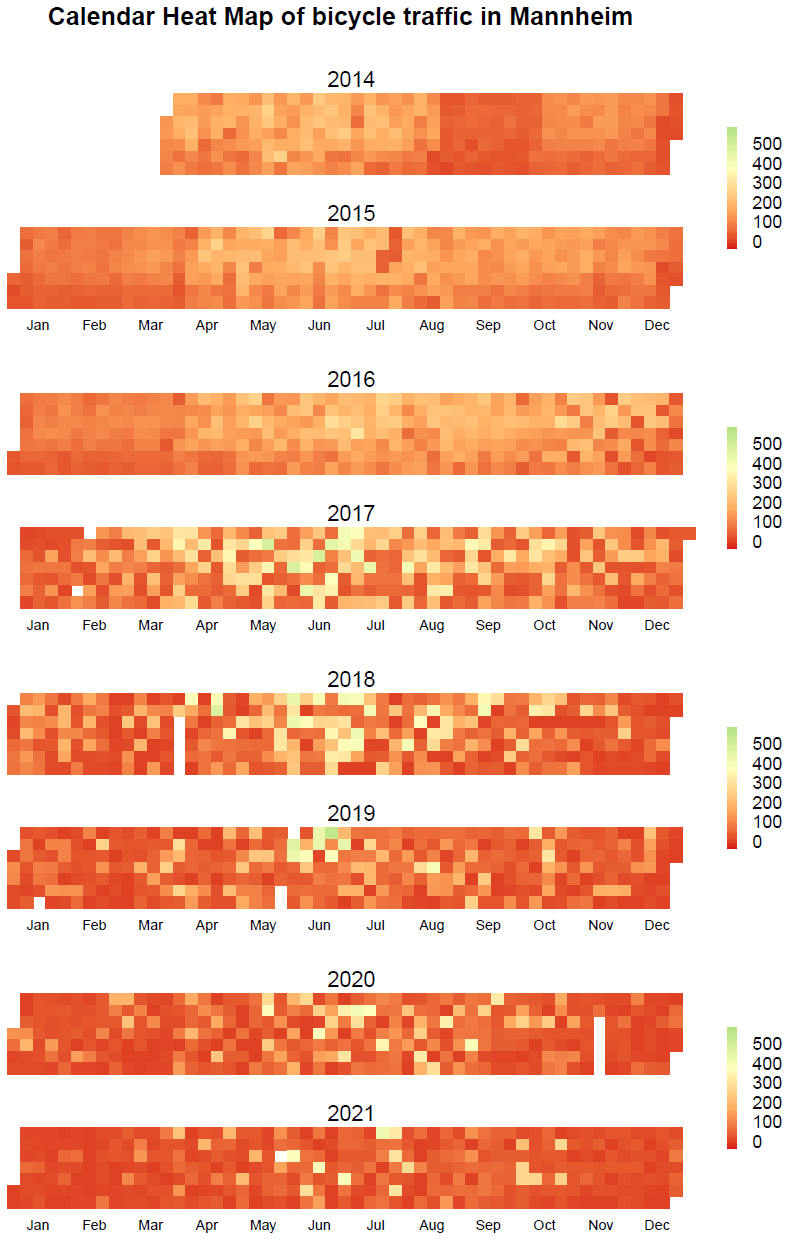
\includegraphics[width=\textwidth]{Plots/CalendarHeatMap.png}
	\captionsource{Korrelations Plot}{
		Korrelation zwischen den verschiedenen Variablen
	}
	\label{fig:meine-grafik5}
\end{figure}

\section{EcoCounter Mannheim}

In Mannheim gibt es 8 verschiedene Stationen. Einen Überblick über diese Stationen ist in Abbildung X zu sehen, wobei zu Erstellung der Graphik ein R Paket genutzt wurde nach \cite{Kahle2013}. Am Farbgradienten ist zu sehen, wie viele Fahrradfahrer pro Stunde die Zählstationen passieren. Zudem ist der Name der Zählstation eingeblendet zudem das Jahr, seitdem diese Zählstation installiert ist. Die älteste Station hier ist die Renzstraße. Jedoch zählte diese während einer Unterbrechung vom ... bis ... nicht.\\
Weiter Variablen wurden aus den Datumsvariabeln erzeugt. So haben wir eine Dummy Variable für Wochenende eingefügt und eine für Sommermonate. Weiterhin nutzen wir Jahr, Monat, Tag und Stunde als Faktorvariablen, wobei wir nächtliche Stunden zwischen 22 und 5 Uhr ausgeschlossen haben.\\
Zu Abweichungen des Fahrradverkehrs konnte es während Corona kommen, wo Teile des öffentlichen Lebens still standen und damit auch das Verkehrsaufkommen. Deshalb haben wir drei Variablen in das Modell aufgenommen.

\begin{figure}[!ht]
	\centering
	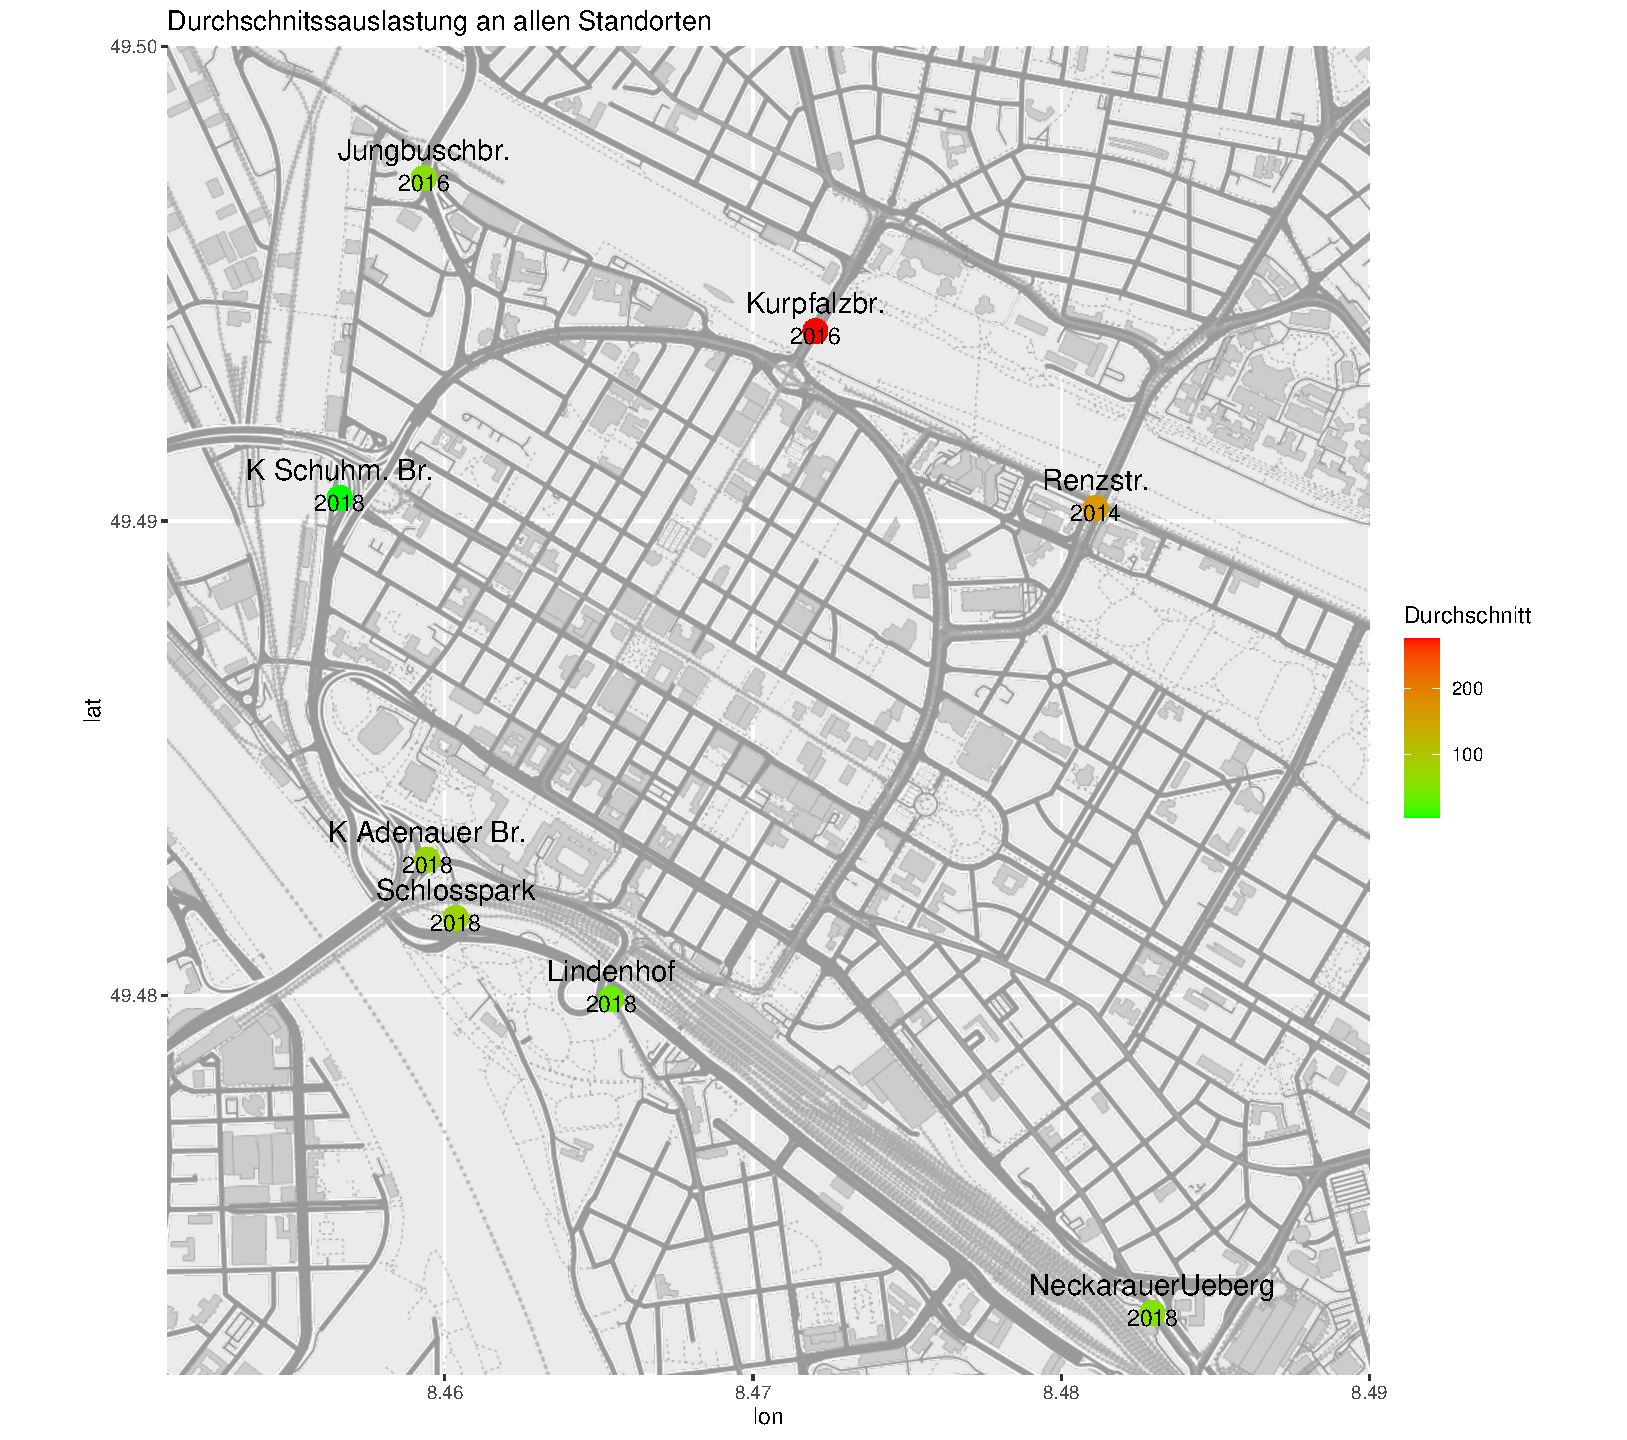
\includegraphics[width=\textwidth]{Plots/Karte_Durchschnittsauslastung.pdf}
	\captionsource{Zählstationsüberblick Mannheim}{
		Zählstation nach Durchschnitt pro Stunde und Startjahr
	}
	\label{fig:meine-grafik5}
\end{figure}



\begin{figure}[!ht]
	\centering
	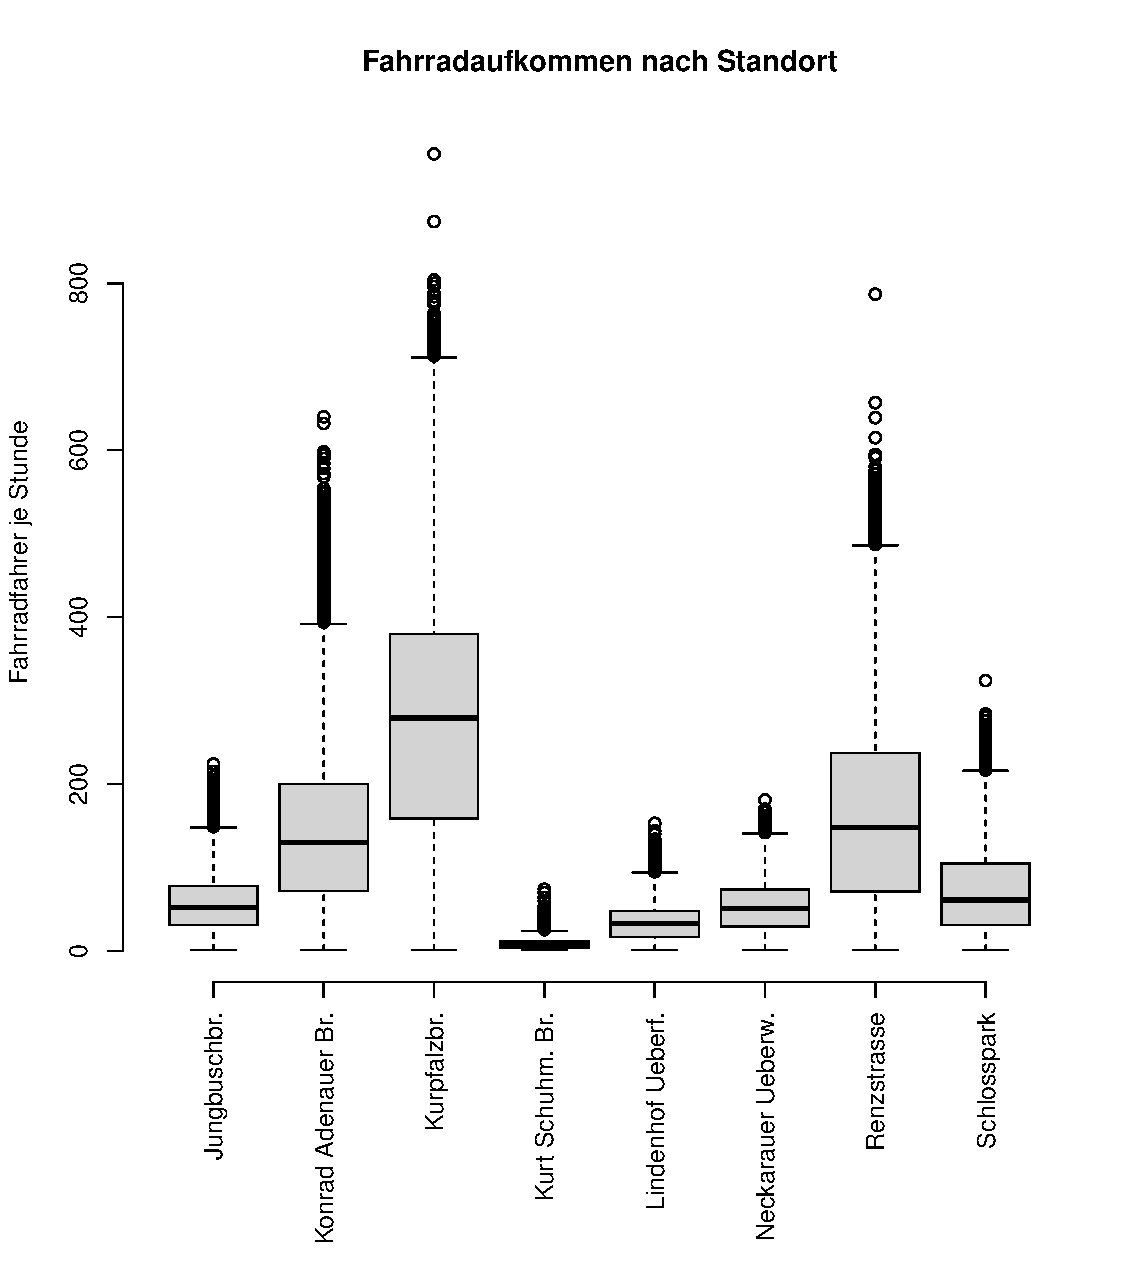
\includegraphics[width=\textwidth]{Plots/Boxplot_Stationen.pdf}
	\captionsource{Boxplots zu den Zählstationen}{
		Verteilung der Fahrräder pro Stunde
	}
	\label{fig:meine-grafik5}
\end{figure}

\section{DWD Daten}


\chapter{Deskriptive Analyse}


\begin{table}[ht]
	\centering
	\begin{tabular}{rllllll}
		\hline
		Name & Min & Durchschnitt & Max & Stand.abw. & Korrelation \\ 
		\hline
		Zaehlstand & 1 & 108.35 & 955 & 120.21 & 1 \\ 
		Distanz z Uni & 208.36 & 1122.51 & 1875.72 & 583.35 & 0.26 \\ 
		Wochenende & 0 & 0.28 & 1 & 0.45 & -0.21 \\ 
		Sommer & 0 & 0.48 & 1 & 0.5 & 0.15 \\ 
		Feiertag BW & 0 & 0.03 & 1 & 0.18 & -0.09 \\ 
		Feiertag RP & 0 & 0.03 & 1 & 0.18 & -0.08 \\ 
		Schulferien BW & 0 & 0.32 & 1 & 0.47 & 0.04 \\ 
		Semesterferien & 0 & 0.48 & 1 & 0.5 & -0.03 \\ 
		WertRR & 0 & 0.07 & 30.4 & 0.49 & -0.03 \\ 
		QualitaetRR & 3 & 3 & 3 & 0 &  \\ 
		WertT2M & -13 & 12.67 & 39.4 & 8.33 & 0.24 \\ 
		QualitaetT2M & 3 & 6.93 & 7 & 0.51 & 0.05 \\ 
		WertF & 0.1 & 3 & 14.4 & 1.65 & -0.02 \\ 
		QualitaetF & 3 & 9.67 & 10 & 1.16 & 0.1 \\ 
		WertRF & 14 & 69.24 & 100 & 20.3 & -0.23 \\ 
		QualitaetRF & 3 & 6.93 & 7 & 0.51 & 0.05 \\ 
		WertSD & 0 & 19.22 & 60 & 24.82 & 0.17 \\ 
		QualitaetSD & 3 & 9.33 & 10 & 1.42 & 0.1 \\ 
		WertN & 0 & 5.72 & 8 & 3.14 & -0.08 \\ 
		QualitaetN & 3 & 3 & 3 & 0 &  \\ 
		Corona & 0 & 0.42 & 1 & 0.49 & -0.16 \\ 
		Kontaktbeschr & 0 & 0.11 & 1 & 0.32 & -0.09 \\ 
		TagesAusbr & 0 & 143.48 & 687 & 212.5 & -0.17 \\ 
		\hline
	\end{tabular}
\end{table}

Notiz für später: Am besten wertest du die Qualitätsdaten genauer aus.


\section{Regressionsanalyse}

\chapter{Einfluss des VRnextbike Angebots}

\chapter{Fazit}

\chapter{Anhang}

\begin{figure}[!ht]
	\centering
	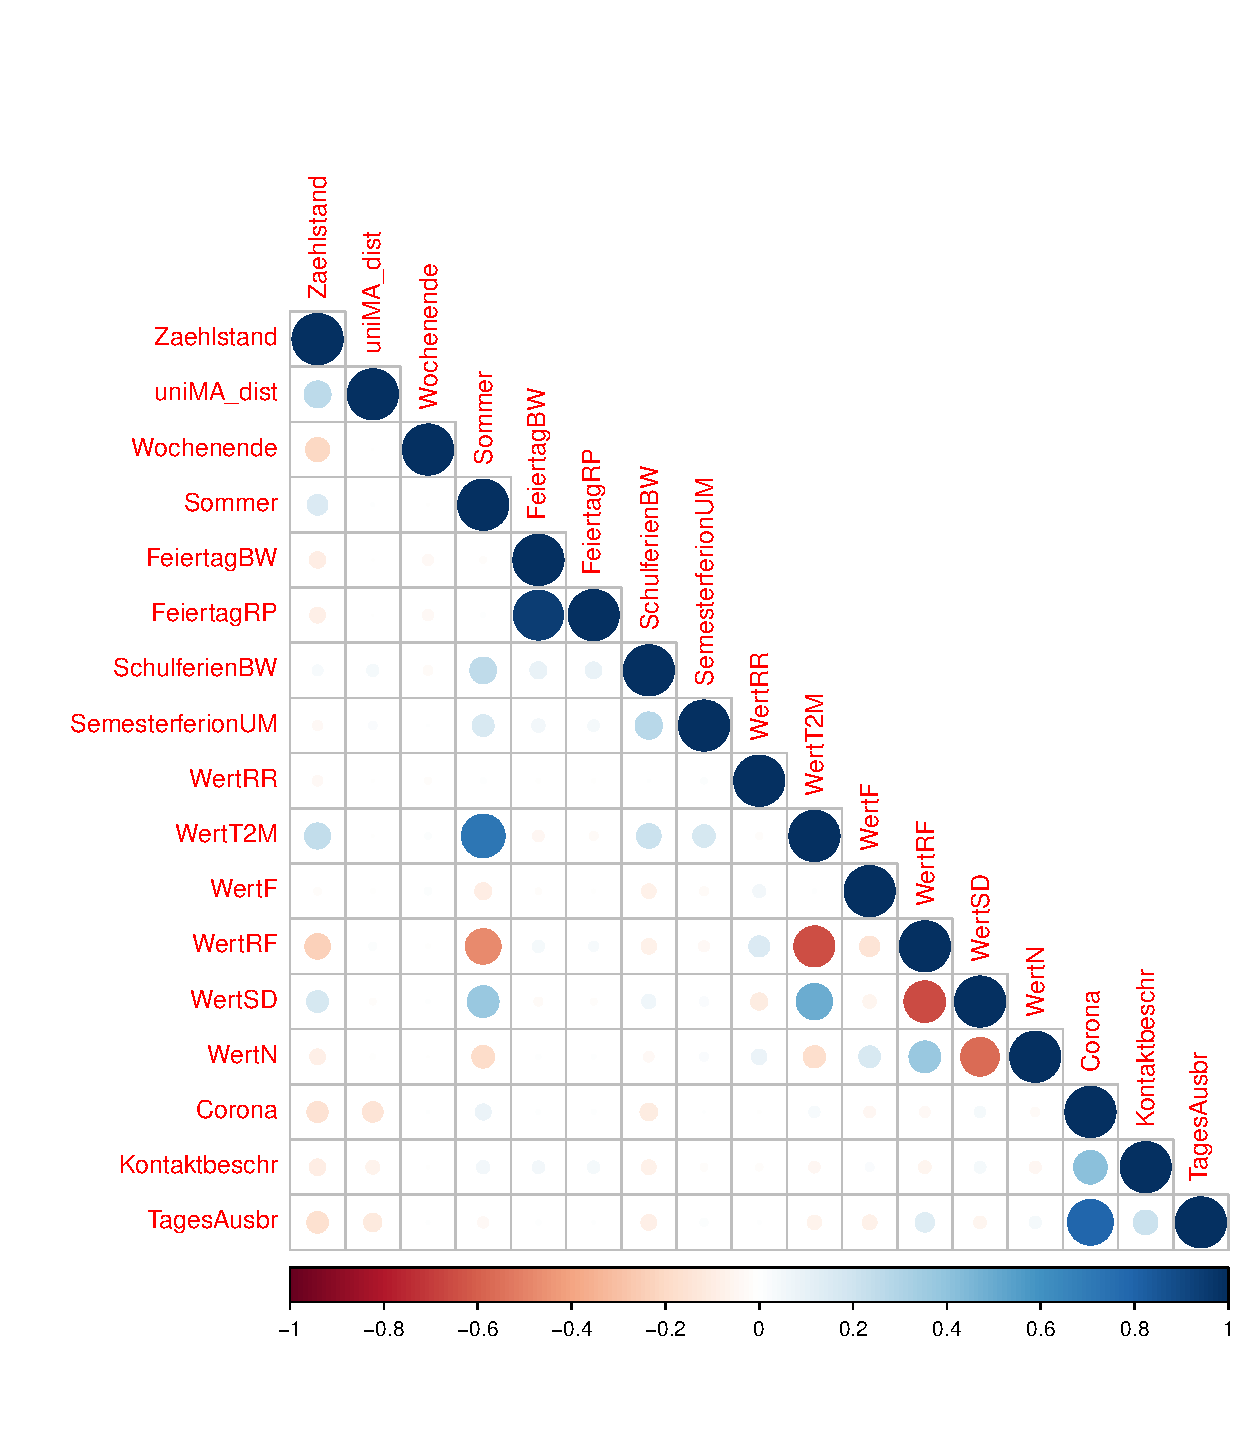
\includegraphics[width=\textwidth]{Plots/Corr_Plot.pdf}
	\captionsource{Korrelations Plot}{
		Korrelation zwischen den verschiedenen Variablen
	}
	\label{fig:meine-grafik5}
\end{figure}

\begin{figure}[!ht]
	\centering
	\includegraphics[width=\textwidth]{Plots/Monatliche_Temperatur_Niederschläge.png}
	\captionsource{Monatliche Durchschnittliche Temperaturen und maximale Niederschläge nach Tageszeiten in 2018}{
		DWD, eigene Darstellung
	}
	\label{fig:meine-grafik5}
\end{figure}

\begin{figure}[!ht]
	\centering
	\includegraphics[width=\textwidth]{Plots/Taegliche_Temperatur_Niederschläge.png}
	\captionsource{Tägliche Durchschnitts Temperaturen und monatliche maximale Niederschläge nach Tageszeiten in 2018}{
		DWD, eigene Darstellung
	}
	\label{fig:meine-grafik5}
\end{figure}

\newpage
\addcontentsline{toc}{chapter}{Literaturverzeichnis}
\bibliography{bib1}

\end{document}
